\section{Efektivitātes atkarība no parametriem}
\subsection{Saules paneļa tipa} \label{subsection:tipi}

Pēc tabulām \ref{tab:JA} un \ref{tab:LG}, kā arī grafikiem, kas ietverti diskusijā par citu parametru ietekmi uz efektivitāti (skat. \ref{subsection:gads}. nod.), redzams, ka LG tipa paneļi konsekventi ir efektīvāki par JA tipu. Tas ir saistīts gan ar kristāla veidu -- kā parādīts \ref{section:tipi}. nod.,  monokristāliska Si paneļi ir ražīgāki par polikristāliem --, gan paneļu maksimālajām jaudām -- LG
ir lielāka nominālā jauda uz laukuma vienību nekā JA.

\begin{table}[!htbp]
    \caption{JA tipa paneļu saražotā enerģija uz kvadrātmetru salīdzināta ar\\ enerģijas plūsmas blūvumu uz horizontālu virsmu}
    \begin{center}
    %%%%%%%%%%%%%%%%%%%%%%%%%%%%%%%%%%%%%%%%%%%%%%%%%%%%%%%%%%%%%%%%%%%%%%
%%                                                                  %%
%%  This is a LaTeX2e table fragment exported from Gnumeric.        %%
%%                                                                  %%
%%%%%%%%%%%%%%%%%%%%%%%%%%%%%%%%%%%%%%%%%%%%%%%%%%%%%%%%%%%%%%%%%%%%%%
\begin{tabular}{ | c | r r r r r  r | } \hline
E, $\textrm{kWhm}^{-2}$	&A.13	&R.13	&D.13	&D.40	&D.90	&piranometrs\\ \hline
jan		&0.35	&0.23	&0.72	&2.46	&2.80		&12.14\\
feb		&3.20	&2.74	&4.27	&6.45	&5.99		&25.14\\
mar		&8.22	&7.40	&9.47	&11.94	&8.72		&61.76\\
apr		&19.89	&19.23	&23.27	&25.43	&18.25		&141.41\\ \hline
$E_{sum}$, $\textrm{kWhm}^{-2}$
		&31.7	&29.6	&37.7	&46.3	&35.8 	&240.5\\ \hline
\end{tabular}
    \end{center} \label{tab:JA}
\end{table}
\begin{table}[!htbp]
    \caption{LG tipa paneļu saražotā enerģija uz kvadrātmetru salīdzināta ar\\ enerģijas plūsmas blūvumu uz horizontālu virsmu}
    \begin{center}
    %%%%%%%%%%%%%%%%%%%%%%%%%%%%%%%%%%%%%%%%%%%%%%%%%%%%%%%%%%%%%%%%%%%%%%
%%                                                                  %%
%%  This is a LaTeX2e table fragment exported from Gnumeric.        %%
%%                                                                  %%
%%%%%%%%%%%%%%%%%%%%%%%%%%%%%%%%%%%%%%%%%%%%%%%%%%%%%%%%%%%%%%%%%%%%%%
\begin{tabular}{ | c | r r r r r  r | } \hline
E, $\textrm{kWhm}^{-2}$	&A.13	&R.13	&D.13	&D.40	&D.90 	&piranometrs\\ \hline
jan	&0.5	&0.35	&0.95	&2.82	&3.22		&12.14	\\
feb	&4.43	&3.63	&5.05	&8.25	&7.41		&25.14	\\
mar	&10.92	&9.27	&11.27	&15.69	&11.34		&61.76	\\
apr	&27.63	&25.46	&29.14	&34.21	&23.18		&141.41	\\ \hline
$E_{sum}$, $\textrm{kWhm}^{-2}$
	&43.48	&38.7	&46.41	&60.98	&45.14		&240.46	\\ \hline
\end{tabular}
    \end{center} \label{tab:LG}
\end{table}

% %%%%%%%%%
\subsection{Saules paneļa leņķa}\label{subsection:degree}
Apkopojot četru mēnešu datus un abus paneļu tipus, visražīgākais leņķis ir 40\textdegree ~(skat.~\ref{fig:lg_ja_deg}. att.).
Kopumā var secināt, ka pret D orientētais panelis 90\textdegree ~leņķī saražo vairāk enerģijas ziemas mēnešos un 13\textdegree ~leņķī -- vasaras mēnešos, tātad apstiprinās teorijā (\ref{section:kustiba}.nod.) prognozētais.
% Tas sakrīt ar [ielikt grafiku ar LV karti un optimālo leņķi bet es neatceros no kurienes paņēmu to].
\begin{figure}[h!]
    \centering
    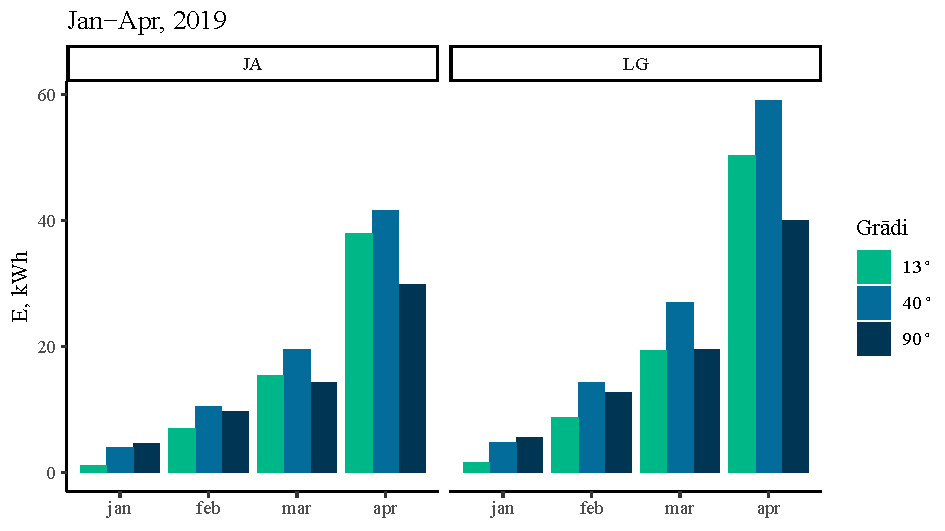
\includegraphics[width=\linewidth]{figures/results/all_degType.pdf}
    \caption{D virzienā vērsto saules paneļu saražotā enerģija atkarībā no leņķa un saules paneļu tipa} \label{fig:lg_ja_deg}
\end{figure}


\subsection{Saules paneļa virziena}\label{subsection:dir}
Visražīgākais virziens ir D, tad A, tad R (skat.~\ref{fig:lg_ja_dir}. att.). To paskaidro \ref{subsection:month_day}. nod. redzamie paneļu saražotās enerģijas dienas sadalījumi.
\begin{figure}[h!]
    \centering
    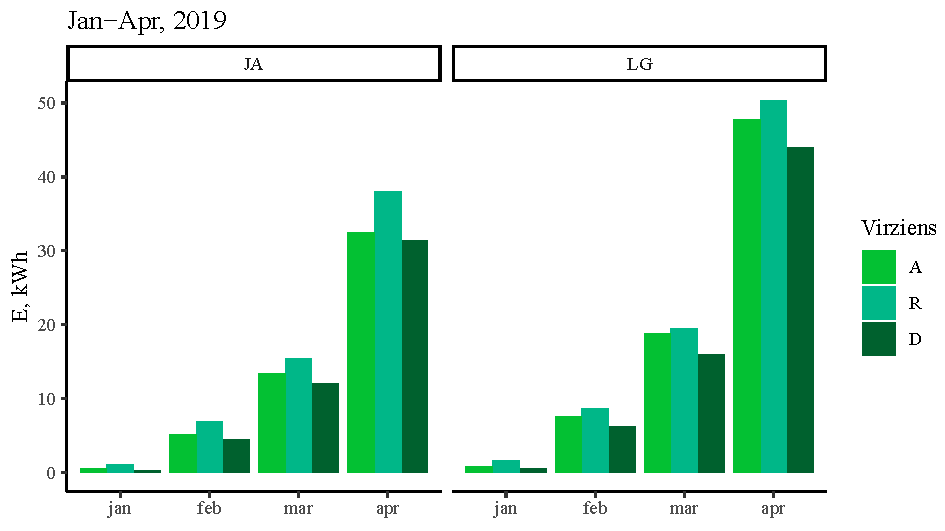
\includegraphics[width=\linewidth]{figures/results/all_dirType.pdf}
    \caption{13 grādu leņķī vērsto saules paneļu atkarība no virziena un saules paneļu tipa}
    \label{fig:lg_ja_dir}
\end{figure}

\subsection{Saules paneļa leņķa un virziena kombinācijas}
\label{subsection:month_day}

Saules paneļu saņemtā apstarojuma dienas sadalījuma tendenci drīkst salīdzināt ar attiecīgo paneļu saražotās enerģijas tendenci, jo pēdējā ir atkarīga no paneļa virsmas saņemtā Saules apstarojuma, kas savukārt ir funkcija no $cos(\theta)$, tātad proporcionāla tam. Salīdzinot \ref{fig:cos-theta}.(c) ar 
\ref{fig:toldU}, tiek secināts, ka eksperimentālie rezultāti sakrīt ar teoriju.

\begin{figure}[h]
    \centering
    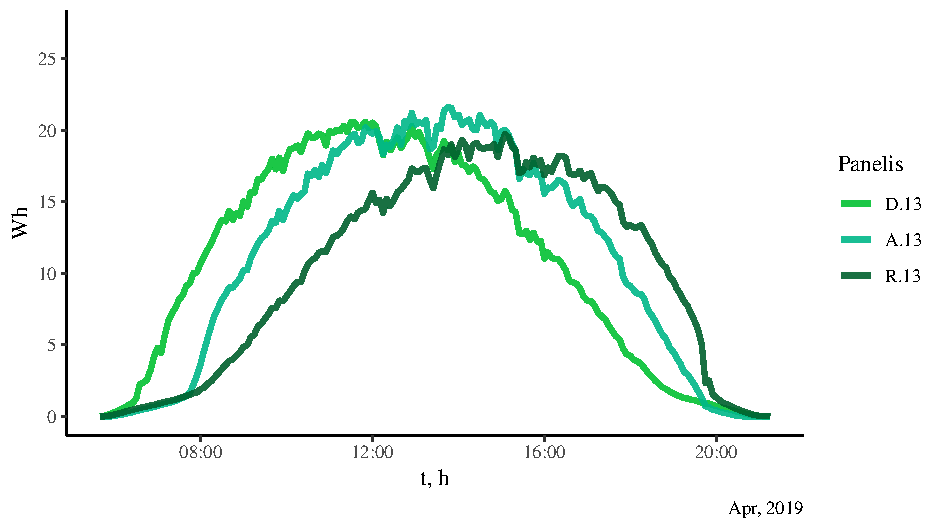
\includegraphics[width=\linewidth]{figures/sol_day/apr_LG_13.pdf}
    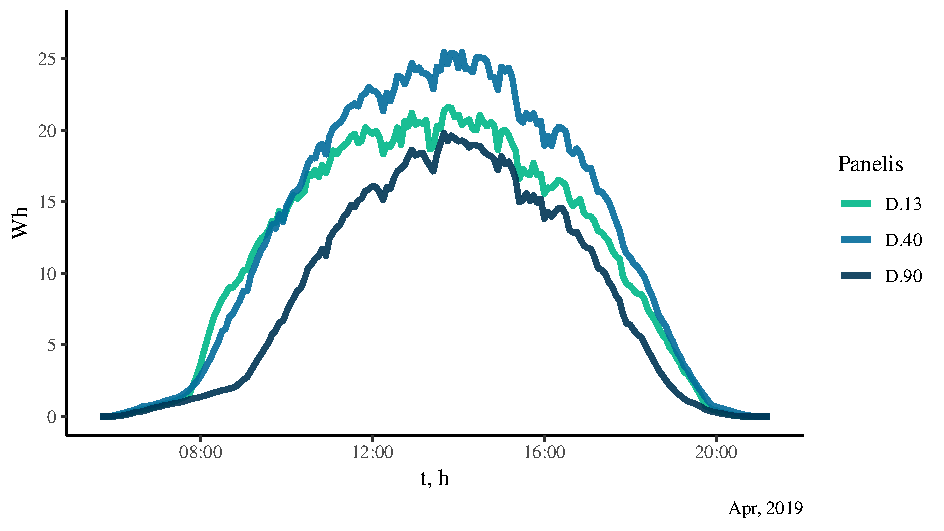
\includegraphics[width=\linewidth]{figures/sol_day/apr_LG_D.pdf}
    \caption{Saules paneļu saražotās enerģijas dienas sadalījuma līkne vidējotiem 27-30. aprīļa datiem} \label{fig:toldU}
\end{figure}

Turpmāk apskatīts Saules apstarojuma dienas sadalījums mēnešos. Kā redzams \ref{fig:mar_ar}, \ref{fig:apr_ar}. att., eksperimentāli noteiktais saules paneļu saražotās enerģijas dienas sadalījums sakrīt ar teorētiski prognozēto \ref{fig:cos-theta}. att. kā arī labi novērojamas tā diennakts svārstības 30 dienu laikā.
% \begin{figure}[h]
%     \centering
%     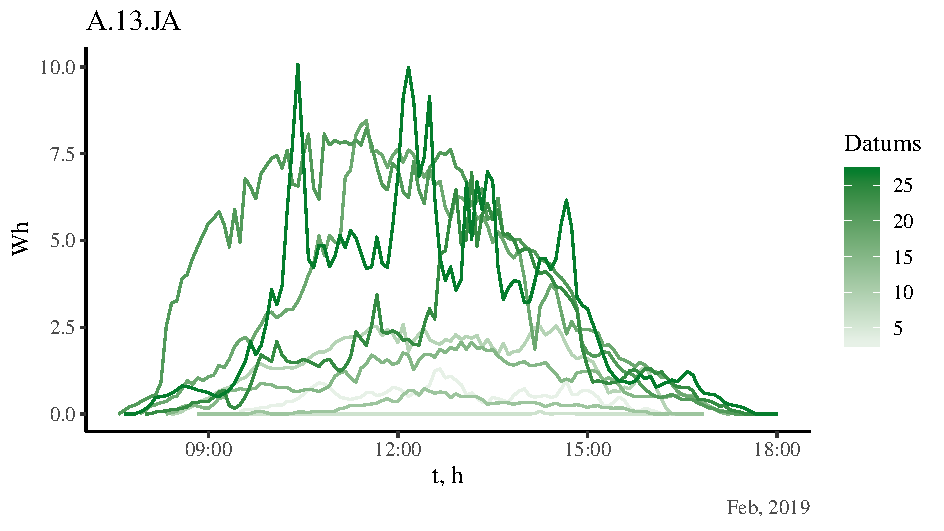
\includegraphics[width=\linewidth]{figures/sol_day/feb_A13JA.pdf}
%     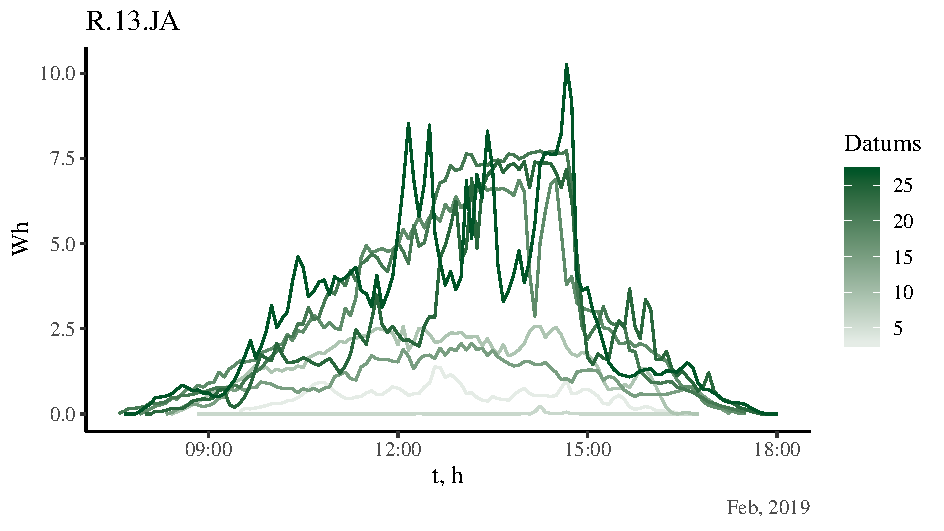
\includegraphics[width=\linewidth]{figures/sol_day/feb_R13JA.pdf}
%     \caption{A un R virzienu saules paneļu 5 minūtēs vidējotu Wh dienas sadalījumi februārī}
%     \label{fig:feb_ar}
% \end{figure}

\begin{figure}[h]
    \centering
    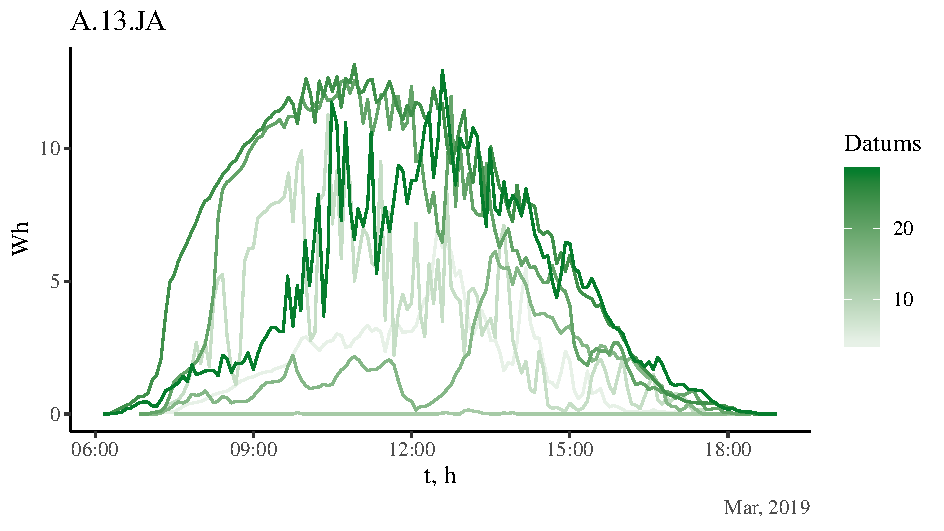
\includegraphics[width=\linewidth]{figures/sol_day/mar_A13JA.pdf}
    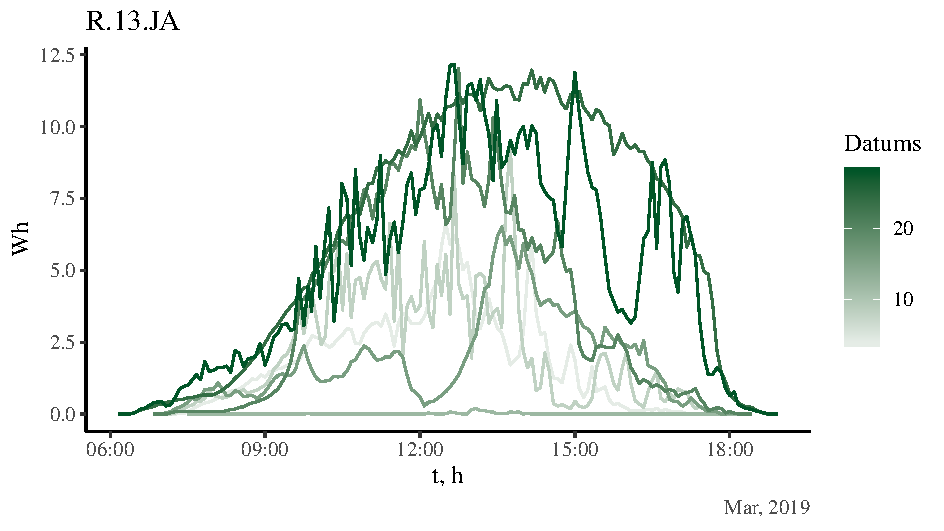
\includegraphics[width=\linewidth]{figures/sol_day/mar_R13JA.pdf}
    \caption{A un R virzienu saules paneļu 5 min intervālos integrētu jaudu dienas sadalījumi martā}
    \label{fig:mar_ar}
\end{figure}

\begin{figure}[h]
    \centering
    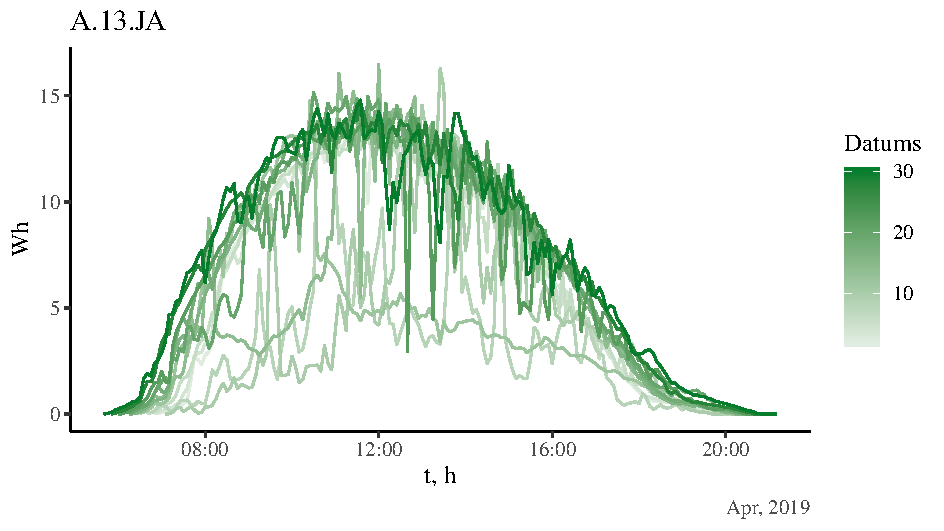
\includegraphics[width=\linewidth]{figures/sol_day/apr_A13JA.pdf}
    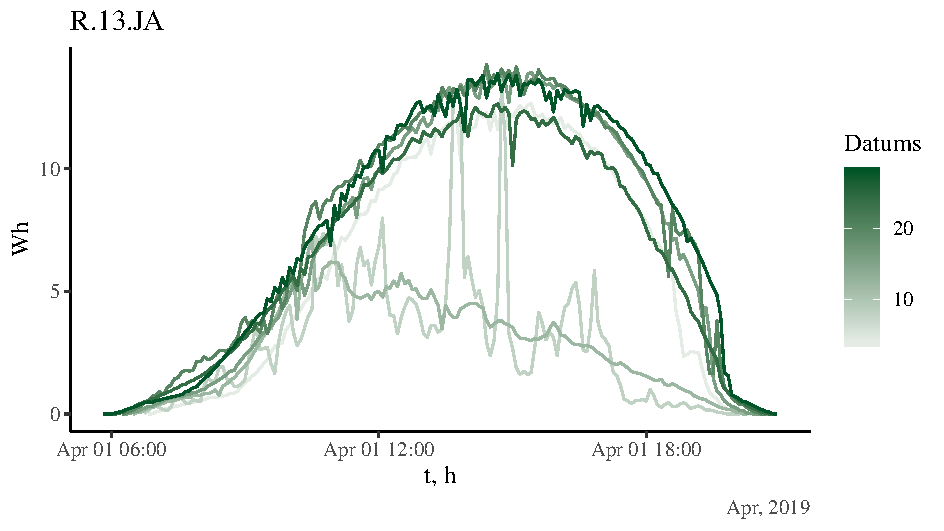
\includegraphics[width=\linewidth]{figures/sol_day/apr_R13JA.pdf}
    \caption{A un R virzienu saules paneļu 5 minūtēs vidējotu Wh dienas sadalījumi aprīlī}
    \label{fig:apr_ar}
\end{figure}

% % \begin{figure}[h]
% %     \centering
% %     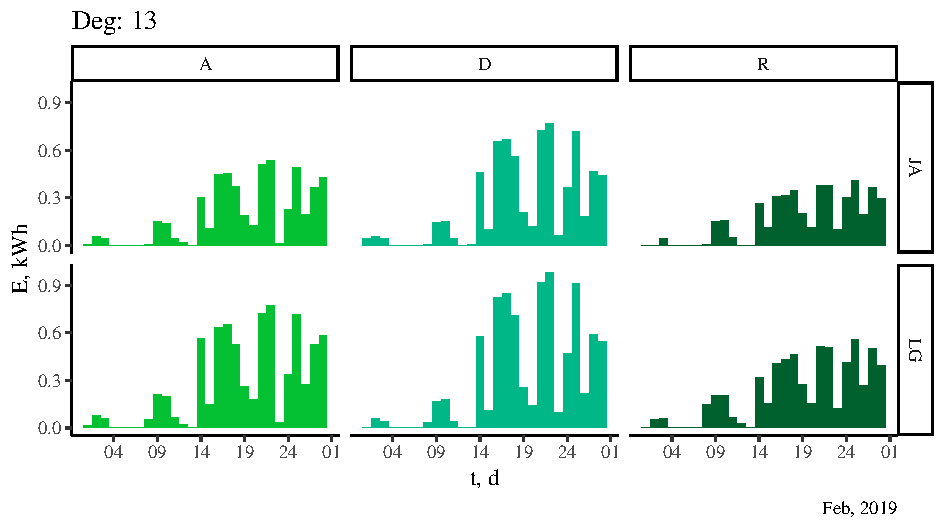
\includegraphics[width=\linewidth]{figures/sol_month/feb_Dir_d.pdf}
% %     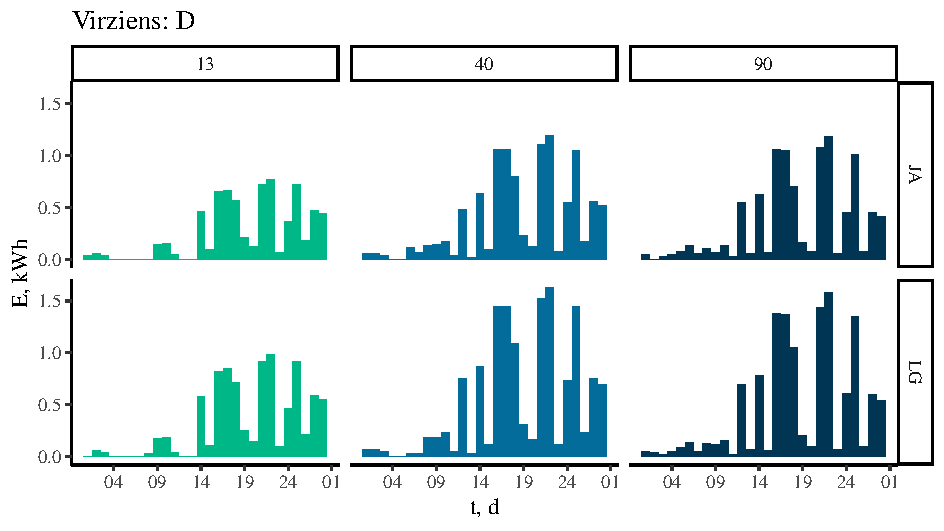
\includegraphics[width=\linewidth]{figures/sol_month/feb_Deg_d.pdf}
% %     \caption{Saules paneļu saražotā enerģija atkarībā no virziena un leņķa februārī}
% %     \label{fig:feb_degDir}
% % \end{figure}

% % \begin{figure}[h]
% %     \centering
% %     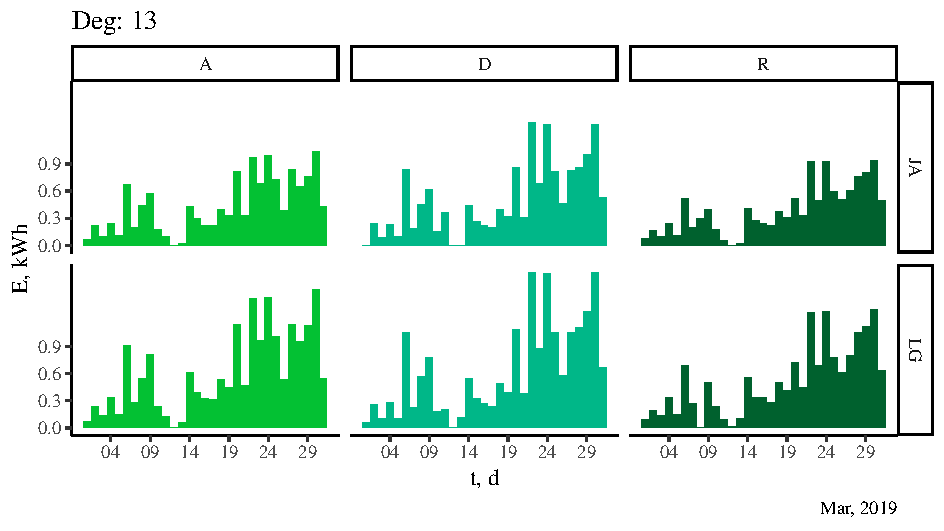
\includegraphics[width=\linewidth]{figures/sol_month/mar_Dir_d.pdf}
% %     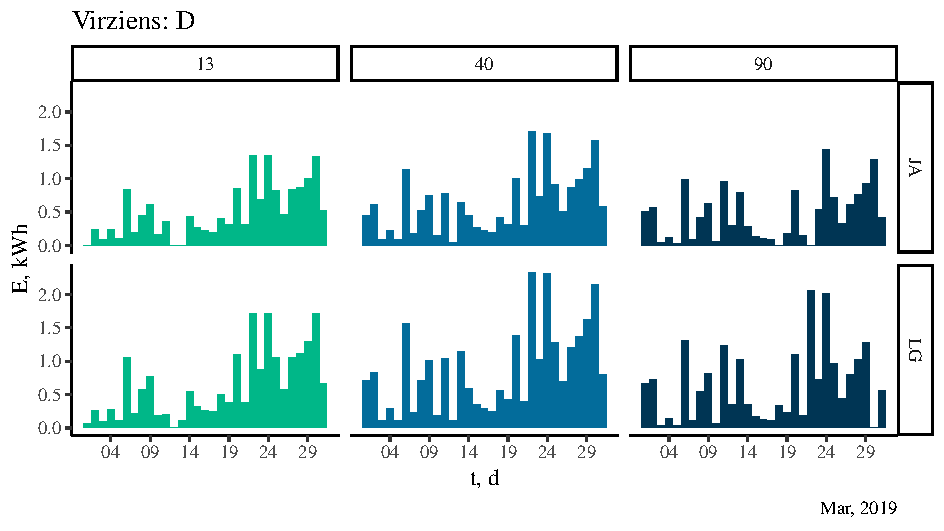
\includegraphics[width=\linewidth]{figures/sol_month/mar_Deg_d.pdf}
% %     \caption{Saules paneļu saražotā enerģija atkarībā no virziena un leņķa martā}
% %     \label{fig:mar_degDir}
% % \end{figure}

% % \begin{figure}[h]
% %     \centering
% %     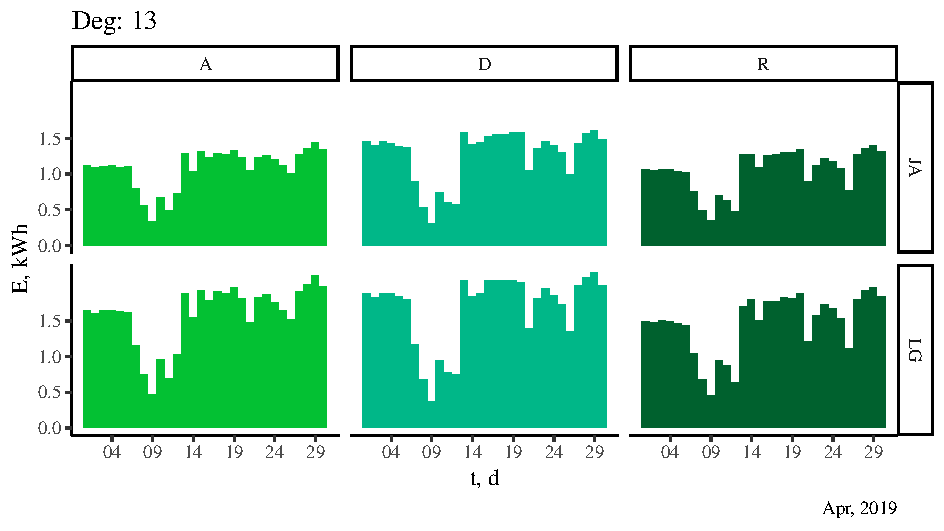
\includegraphics[width=\linewidth]{figures/sol_month/apr_Dir_d.pdf}
% %     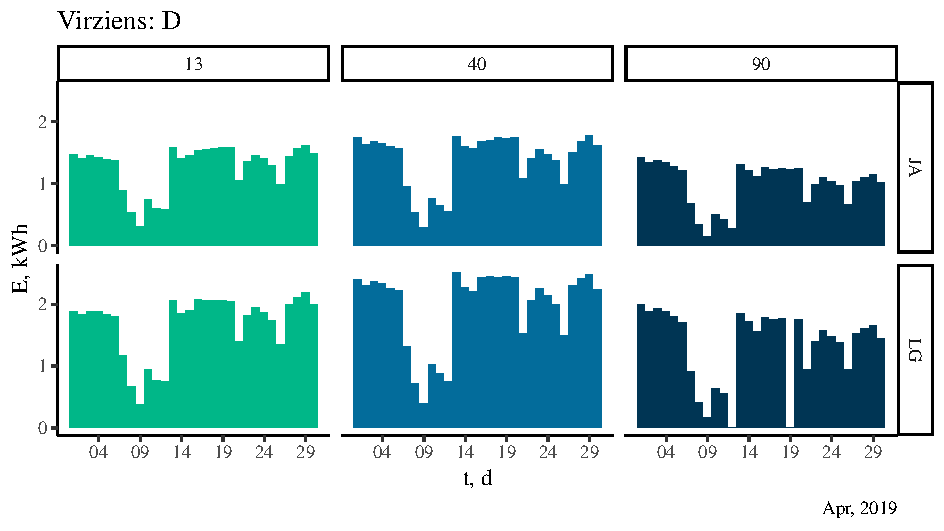
\includegraphics[width=\linewidth]{figures/sol_month/apr_Deg_d.pdf}
% %     \caption{Saules paneļu saražotā enerģija atkarībā no virziena un leņķa aprīlī}
% %     \label{fig:apr_degDir}
% % \end{figure}

\subsection{Gada mēneša} \label{subsection:gads}
Pēc \ref{fig:jan_sum}, \ref{fig:feb_sum}, \ref{fig:mar_sum}, \ref{fig:apr_sum}. att., tiek izdarīti secinājumi par saules paneļu ražīguma atkarību no gada mēneša. Janvārī visefektīvākais panelis ir D.90, kas atbilst janvārim raksturīgajam Saules pārvietojumam -- zemu pie horzionta. \ref{fig:feb_sum}. att. redzams, ka februārī D.40 kļūst ražīgāks nekā D.90, tāpat redzams, ka mazāku leņķu paneļi -- R.13 un A.13 -- proporcionali vairāk Saules apstarojuma ir pārvērtuši enerģijā. Šī tendence novērojama arī turpmākajos mēnešos. Savukārt jau aprīlī visefektīvākā orientācija ir D.40. Visu telpisko orientāciju paneļi ir pakļauti Saules diennakts pārvietojuma izmaiņas izraisītajiem efektiem uz saražotās enerģijas apjomu, kas teorētiski aprēķināti \ref{section:kustiba}. nod.

% Janvārī visefektīvākaie ir paneļi, kas orientēti uz dienvidiem un novietoti vertikāli (D.90), jo Saule pārvietojas zemu gar horizontu. Savukārt jau aprīlī visefektīvākā orientācija ir D.40, un arī citu orientāciju paneļi ir pakļaut līdzīgiem efektiem, kas teorētiski aprēķināti \ref{section:kustiba}. nod.

Arī Ulbrokas saules paneļu spēkstacijas darbības analīze gada griezumā (skat. \ref{fig:ulbroka}. att.) uzrāda ļoti būtisku saules paneļu saražotās enerģijas variabilitāti gada mēnešos. Maksimālais enerģijas daudzums tiek saražots maijā, nedaudz mazāk citos vasaras mēnešos, bet janvārī, februārī, novembrī un decembrī saražotās enerģijas daudzums ir ļoti mazs. Šis apsvērums ir īpaši svarīgs industrializētos pielietojumos, jo ziemas mēnešos jādomā par alternatīvu enerģijas avotu.

\begin{figure}[h]
    \centering
    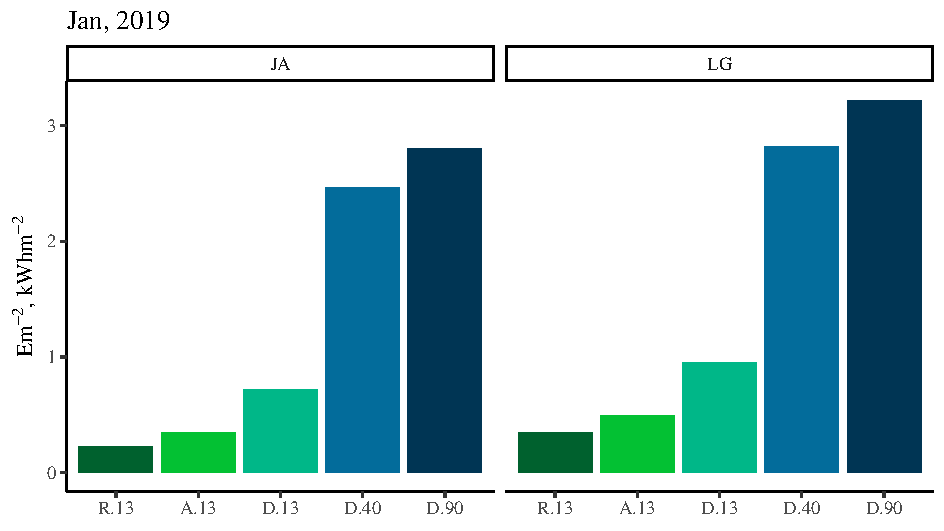
\includegraphics[width=\linewidth]{figures/sol_month/jan_m_m2.pdf}
    \caption{Saules paneļu saražotā enerģija janvārī}
    \label{fig:jan_sum}
\end{figure}

\begin{figure}[h]
    \centering
    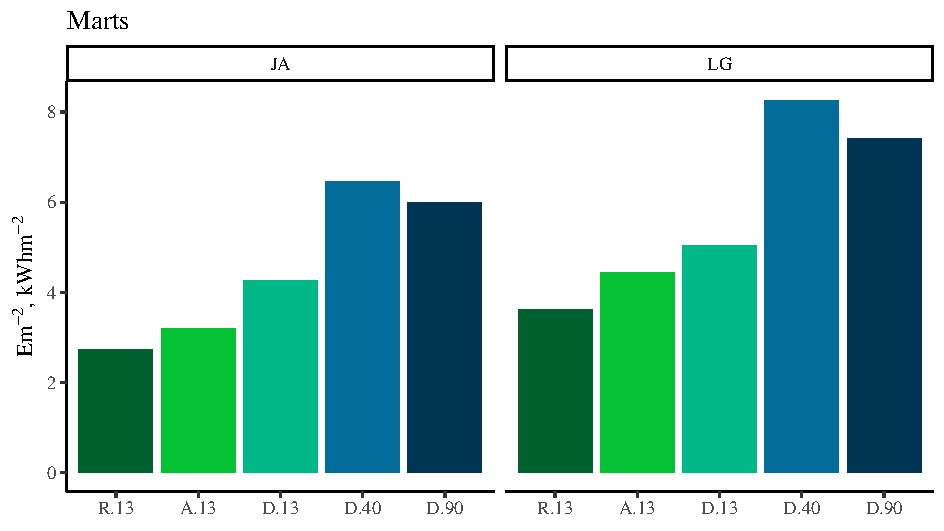
\includegraphics[width=\linewidth]{figures/sol_month/feb_m_m2.pdf}
    \caption{Saules paneļu saražotā enerģija februārī}
    \label{fig:feb_sum}
\end{figure}

\begin{figure}[h]
    \centering
    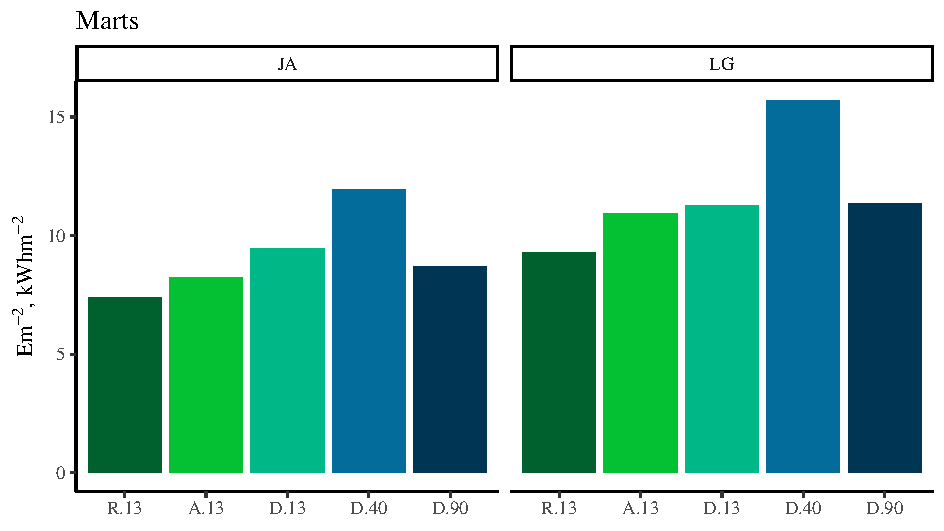
\includegraphics[width=\linewidth]{figures/sol_month/mar_m_m2.pdf}
    \caption{Saules paneļu saražotā enerģija martā}
    \label{fig:mar_sum}
\end{figure}

\begin{figure}[h]
    \centering
    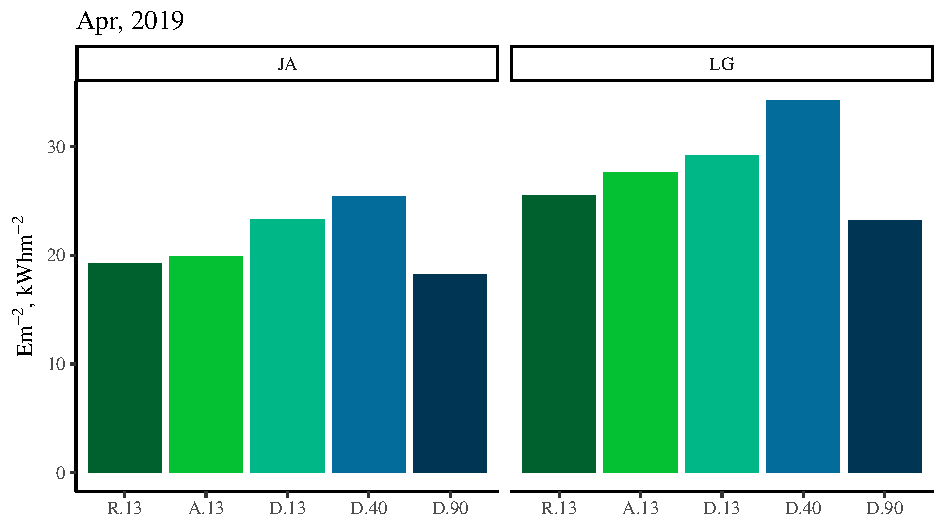
\includegraphics[width=\linewidth]{figures/sol_month/apr_m_m2.pdf}
    \caption{Saules paneļu saražotā enerģija aprīlī}
    \label{fig:apr_sum}
\end{figure}


\section{Salīdzinošā analīze}\label{section:effectivity}

Eksperimentāli noteiktā paneļu efektivitāte (skat.~\ref{tab:eff_type}. tab.) nav pretrunā ne ar ražotāju tehniskajā dokumentācijā doto, nedz teorētiski iespējamo pēc S-Q modeļa. 
% Izmērītā paneļu efektivitāte atšķiras no ražotāju tehniskajā dokumentācijā dotā.
Atšķirības tiek skaidrotas ar efektivitātes mērīšanas veidu -- standarta testi tiek veikti pie konstanta izstarojuma (1000 W/m$^2$ un 800 W/m$^2$) perpendikulāri saules panelim, tomēr reālā poligona apstākļos novērojama starojuma avota kustība pa debesjumu gan diennakts, gan gada ietvaros.

\begin{table}[h!]
    \caption{Katra paneļa eksperimentāli noteiktās efektivitātes vidējā vērtība 4 mēnešu laikā}
    \begin{center}
    %%%%%%%%%%%%%%%%%%%%%%%%%%%%%%%%%%%%%%%%%%%%%%%%%%%%%%%%%%%%%%%%%%%%%%
%%                                                                  %%
%%  This is a LaTeX2e table fragment exported from Gnumeric.        %%
%%                                                                  %%
%%%%%%%%%%%%%%%%%%%%%%%%%%%%%%%%%%%%%%%%%%%%%%%%%%%%%%%%%%%%%%%%%%%%%%
\begin{tabular}{ | c | c c c c c | }\hline
Panelis	&A.13	&R.13	&D.13	&D.40	&D.90\\ \hline
E$_{JA}$, \%		&0.11	&0.10	&0.14	&0.21	&0.18\\ \hline
E$_{LG}$, \%		&0.15	&0.13	&0.17	&0.26	&0.23\\ \hline
\end{tabular}
    \end{center}
    \label{tab:eff_type}
\end{table}

\begin{figure}[h!]
    \centering
    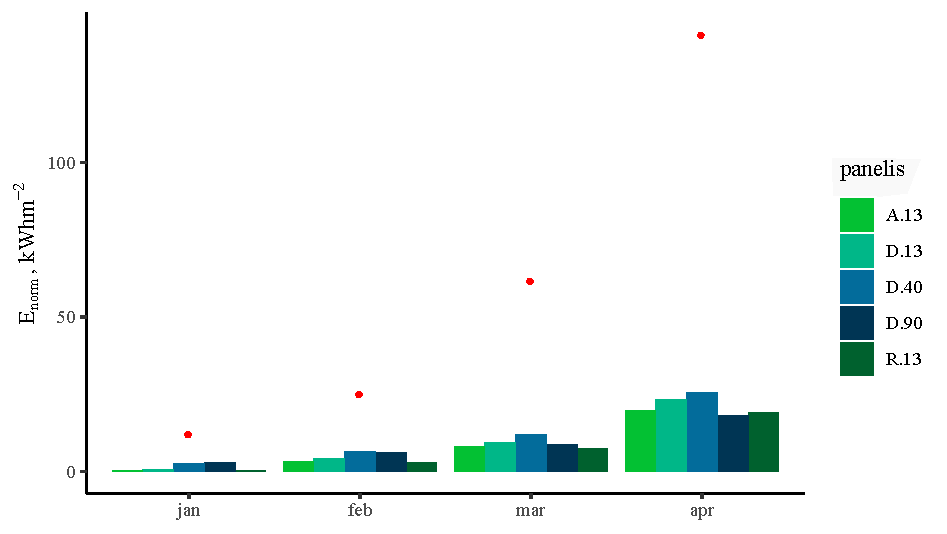
\includegraphics[width=\linewidth]{figures/results/JAm2_w.pdf}
    \caption{JA tipa paneļu saražotais mēnesī salīdzinājumā ar eksperimentālā poligona meteostacijas saules apstarojuma datiem uz horizontālu virsmu (\textcolor{bostonuniversityred}{sarkanā krāsā})}
    \label{fig:ja}
\end{figure}
\begin{figure}[h!]
    \centering
    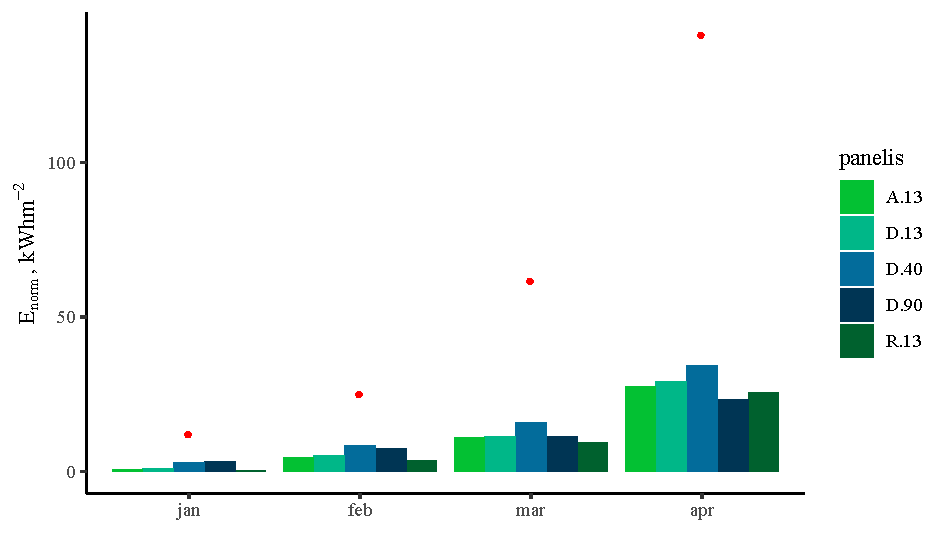
\includegraphics[width=\linewidth]{figures/results/LGm2_w.pdf}
    \caption{LG tipa paneļu saražotais mēnesī salīdzinājumā ar eksperimentālā poligona meteostacijas saules apstarojuma datiem uz horizontālu virsmu (\textcolor{bostonuniversityred}{sarkanā krāsā})}
    \label{fig:lg}
\end{figure}

\section{Salīdzinājums ar citas saules paneļu spēkstacijas mērījumu rezultātiem}

Tabulās \ref{tab:ja_ul}. un \ref{tab:lg_ul} salīdzināta Botānisko dārzu saules paneļu saražotā enerģija 2019. gada janvārī -- aprīlī ar 2017. gada Ulbrokas spēkstacijas viena paneļa saražoto enerģiju janvāra -- aprīļa periodā. Jāpiebilst, ka spēkstacijām atšķiras lokācijas, turklāt, spriežot pēc, \ref{fig:metYears_mean}. att., 2019. gadā attiecīgajos mēnešos bija krietni lielāks Saules apstarojums, kas izskaidro Ulbrokas paneļu šķietamo neefektivitāti, taču dod ieskatu sistēmas prognozējamā darbībā.
\begin{table}[h]
    \caption{JA tipa paneļu saražotās enerģijas salīdzinājums ar Ulbrokas spēkstacijā saražoto 2017. gadā}
    \begin{center}
    %%%%%%%%%%%%%%%%%%%%%%%%%%%%%%%%%%%%%%%%%%%%%%%%%%%%%%%%%%%%%%%%%%%%%%
%%                                                                  %%
%%  This is a LaTeX2e table fragment exported from Gnumeric.        %%
%%                                                                  %%
%%%%%%%%%%%%%%%%%%%%%%%%%%%%%%%%%%%%%%%%%%%%%%%%%%%%%%%%%%%%%%%%%%%%%%
\begin{tabular}{ | c | c c c c c c | }\hline
E, kWh	&A.13	&R.13	&D.13	&D.40	&D.90 &Ulbroka\\ \hline
jan	&0.57	&0.37	&1.17	&4.02	&4.58	&0.84\\
feb	&5.23	&4.48	&6.98	&10.54	&9.79	&5.62\\
mar	&13.44	&12.1	&15.49	&19.52	&14.26	&15.59\\
apr	&32.52	&31.44	&38.05	&41.57	&29.84	&25.56\\ \hline
E$_{sum}$, kWh	&51.76	&48.4	&61.68	&75.66	&58.47	&47.61\\ \hline
\end{tabular}
    \end{center} \label{tab:ja_ul}
\end{table}
\begin{table}[h]
    \caption{LG tipa paneļu saražotās enerģijas salīdzinājums ar Ulbrokas spēkstacijā saražoto 2017. gadā}
    \begin{center}
    %%%%%%%%%%%%%%%%%%%%%%%%%%%%%%%%%%%%%%%%%%%%%%%%%%%%%%%%%%%%%%%%%%%%%%
%%                                                                  %%
%%  This is a LaTeX2e table fragment exported from Gnumeric.        %%
%%                                                                  %%
%%%%%%%%%%%%%%%%%%%%%%%%%%%%%%%%%%%%%%%%%%%%%%%%%%%%%%%%%%%%%%%%%%%%%%
\begin{tabular}{ | c | c c c c c c | }\hline
E, kWh	&A.13	&R.13	&D.13	&D.40	&D.90 &Ulbroka\\ \hline
jan	&0.86	&0.60	&1.64	&4.87	&5.55	&0.84\\
feb	&7.65	&6.26	&8.72	&14.26	&12.80	&5.62\\
mar	&18.86	&16.01	&19.47	&27.11	&19.58	&15.59\\
apr	&47.73	&43.97	&50.32	&59.09	&40.03	&25.56\\ \hline
E$_{sum}$, kWh	&75.09	&66.85	&80.15	&105.32	&77.97	&47.61\\ \hline
\end{tabular}
    \end{center}\label{tab:lg_ul}
\end{table}